\chapter{Thermodynamics}
强度量:与物质的量无关的物理量,压力$ p $,温度$ T $。

广延量:与物质的量\textbf{有关}的物理量,具有可加性,质量$ m $,容积$ V $,内能$ E $,焓$ H $,熵$ S $。

比参数:将广延量化为强度量,让其与物质的量无关,方便比较。

\section{能量传递基本概念和状态方程}

经典理想气体状态方程:
\begin{equation}
\label{idealGas}
pV=nRT
\end{equation}

从\autoref{idealGas}推导出\textbf{理想气体密度公式}:
\begin{equation}
\rho = \frac{Mp}{RT} = \frac{p}{R_s T}
\end{equation}

对理想气体而言,各物理性质是压力$ p $和温度$ T $的函数,如$ \rho(p,T) $、$ c_p(p,T) $、$ \mu(T) $、$ k(T) $。

比气体常数(Specific gas constant):
\begin{gather}
R_s = \frac{R}{M} \\
R_s = c_p - c_v
\end{gather}

定压比热容$ c_p $,令的$ 1\si{\kilogram} $物质的温度上升$ 1\si{\kelvin} $所需的能量,单位\si{\joule\per\kilogram\per\kelvin}。

比热容比(The ratio of specific thermal capacities),常见的双原子气体的$ \gamma=1.4 $,大多数液体的$ \gamma=1.1 $,水的$ \gamma=1.0 $。
\begin{equation}
\gamma = \frac{c_p}{c_v}
\end{equation}

热扩散系数(Thermal diffusivity, \si{\meter\squared\per\second}),其中$ k $为热导率( \si{\watt\per\meter\per\kelvin}),$ \rho $为密度( \si{\kilogram\per\cubic\meter}),$ c_p $为定压比热容(\si{\joule\per\kilogram\per\kelvin})。其用于评估材料导热能力相对于储热能力的大小,$ \alpha $越大,导热能力越强。

\begin{equation}
\alpha = \frac{k}{\rho c_p}
\end{equation}

焦耳:

\[1\si{\joule} = 1\si{\newton\meter} = \frac{\si{\kilogram\meter\squared}}{\si{\second\squared}} = 1\si{\watt\second} \]

\[1W = 1\si{\joule\per\second}\]

根据Fourier定律,产热速率$ Q $(\si{\watt}=\si{\joule\per\second})定义为:

\begin{equation}
Q = \propto A \frac{\partial T}{\partial x}
\end{equation}

对于材料属性稳定的材料而言,比例系数是恒定的,将其定义为热导率$ k $(\si{\watt\per\meter\per\kelvin})。负号是因为传热的方向与温度梯度相反:

\begin{equation}
Q = -k A \frac{\partial T}{\partial x}
\end{equation}

热通量定义为单位面积上的传热速率,$ q $(\si{\watt\per\meter\squared}=\si{\joule\per\meter\squared\second}):

\begin{equation}
q = \frac{Q}{A}
\end{equation}

很容易将方程扩展到三维:

\begin{equation}
q = -k\nabla T
\end{equation}

通常,我们希望知道物体的温度分布,即温度在介质中随位置是如何变化的。一旦知道了这种分布,就可以用Fourier定律计算介质中任何一点的导热通量。

考虑一个匀质的介质,其温度分布$ T(x,y,z) $使用Cartesian坐标表示,同时,假定介质是静止且不可压缩的。在介质中定义一个无限小的微元控制体,$ dxdydz $。由于物体是静止的,所以不考虑机械能和系统与环境的做功。一旦物体内存在温度梯度,就会发生热传导,如果已知热通量$ q_x $、$ q_y $、$ q_z $,通过Taylor级数展开可以获取相应面的对面的热通量:

\begin{gather}
q_{x+dx} = q_x + \frac{q_x}{x}dx \\
q_{y+dy} = q_y + \frac{q_y}{y}dy \\
q_{z+dz} = q_z + \frac{q_z}{z}dz
\end{gather}

\begin{figure}
    \centering
    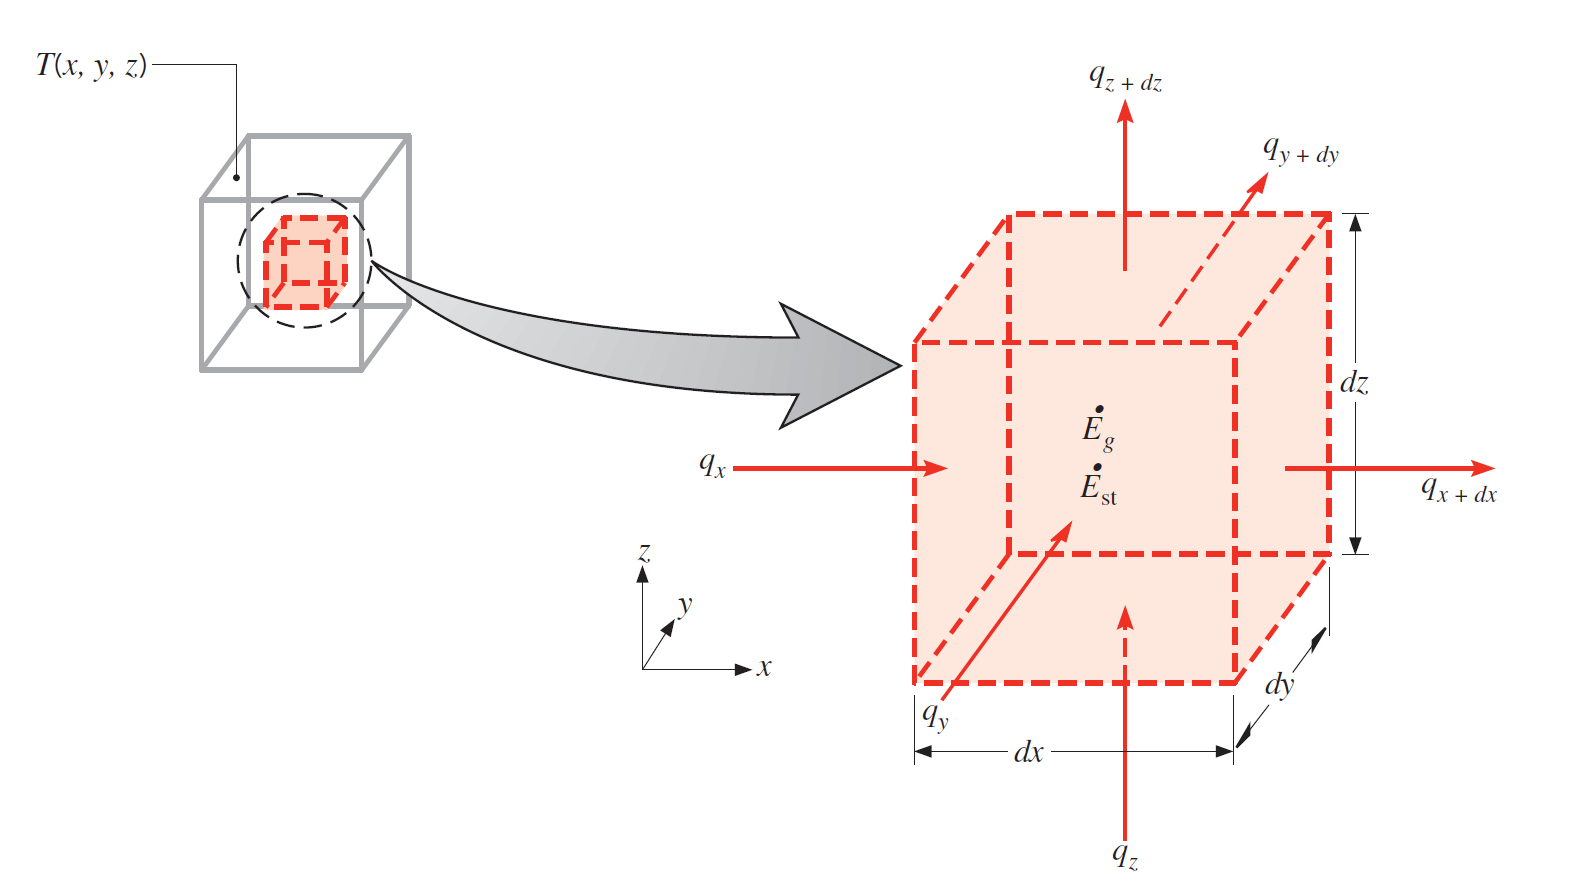
\includegraphics[width=12cm]{heat_conduction}
    \caption{Cartesian坐标系下的微元控制体}
\end{figure}

考虑介质中可能存在的能量源项,其中$ q_g $为单位体积的能力产生速率,(\si{\watt\per\meter\cubed}):

\begin{equation}
E_g = q_g dxdydz
\end{equation}

在介质不发生相变的情况下,不需要考虑潜热,所以介质内能量的变化率为显热(sensible energy)的变化率:

\begin{equation}
E_{cha} = \frac{\partial U_{sens}}{\partial t} = \rho c_v \frac{\partial T}{\partial t}dxdydz = \rho c_p \frac{\partial T}{\partial t}dxdydz
\end{equation}

其中,对不可压缩介质来说,定压比热容和定容比热容相等,$ c_v=c_p $。

将上述方程汇总,写出能量守恒的一般形式,

\begin{gather}
E_{in} - E_{out} + E_g = E_{cha} \\
q_x + q_y + q_z - q_{x+dx} - q_{y+dy} - q_{z+dz} + q_g dxdydz = \rho c_p \frac{\partial T}{\partial t} dxdydz \\
-\frac{\partial q_x}{\partial x} -\frac{\partial q_y}{\partial y} -\frac{\partial q_z}{\partial z} + q_g dxdydz = \rho c_p \frac{\partial T}{\partial t} dxdydz
\end{gather}

考虑材料性质为各向同性,根据Fourier定律来计算热通量:

\begin{gather}
q_x = -k dydz \frac{\partial T}{\partial x} \\
q_y = -k dxdz \frac{\partial T}{\partial y} \\
q_z = -k dxdy \frac{\partial T}{\partial z}
\end{gather}

将上述方程整合,并在两端除以控制体体积$ dxdydz $:

\begin{equation}
\frac{\partial}{\partial x}\left(k\frac{\partial T}{\partial x}\right) + \frac{\partial}{\partial y}\left(k\frac{\partial T}{\partial y}\right) + \frac{\partial}{\partial z}\left(k\frac{\partial T}{\partial z}\right) + q_g = \rho c_p \frac{\partial T}{\partial t}
\end{equation}

为了类比质量扩散方程,定义热扩散系数(thermal diffusivity)为$ \alpha = k/\rho c_p $:

\begin{equation}
\nabla^2 T + \frac{q_g}{k} = \frac{1}{\alpha} \frac{\partial T}{\partial t}
\end{equation}

\section{总能量方程}
能量守恒定义为绝热系统的总能量是一个常数。即总的能量不随时间变化,只能从一种形式转换为另一种形式且不能凭空消失。在CFD里面通常只考虑\textit{动能(机械能)}和\textit{分子内能(内能)}。能量守恒可以表示为:

\begin{center}
\textbf{流体微团内能量的变化率=流入的净热流量+体积力和表面力对微团做功的功率}
\end{center}

动能定义为:

\begin{equation}
K=\frac{1}{2}|\mathbf{u}|^2
\end{equation}

单位质量的内能定义为:$ E $,流体微团动能和内能总和的时间变化率定义为:

\begin{equation}
\rho\frac{D(K+E)}{Dt}dxdydz
\end{equation}

附加热源为$ Q $,流体微团的净热源为:

\begin{equation}
\rho Qdxdydz
\end{equation}

热通量为$ \bm{q}=-k\nabla T $,热传导对流体微团的加热为:

\begin{equation}
-\nabla \cdot\bm{q}dxdydz
\end{equation}

重力做功、压力和剪应力做功可以表示为:

\begin{gather}
\rho\bm{g}\cdot\bm{u}dxdydz \\
(-\nabla\cdot(p\bm{u}) + \nabla\cdot(\tau\cdot\bm{u})) dxdydz
\end{gather}

结合上式,总能量方程为(非守恒形式):

\begin{equation}
\rho\frac{D(K+E)}{Dt} =  -\nabla\cdot(p\bm{u}) + \rho Q - \nabla\cdot\bm{q} + \rho\bm{g}\cdot\bm{u} + \nabla\cdot(\tau\cdot\bm{u})
\end{equation}

总能量方程为(守恒形式):

\begin{equation}
\frac{\partial\rho E}{\partial t} + \frac{\partial\rho K}{\partial t} + \nabla\cdot(\rho\bm{u}E) + \nabla\cdot(\rho\bm{u}K) = -\nabla\cdot(p\bm{u}) + \rho Q - \nabla\cdot\bm{q} + \rho\bm{g}\cdot\bm{u} + \nabla\cdot(\tau\cdot\bm{u})
\end{equation}

\section{内能方程}

抽离动能项后我们能获取一个内能方程。首先,有动量守恒:

\begin{equation}
\rho \frac{D\mathbf{u}}{Dt} = \nabla\cdot\tau + \rho g + \nabla p
\end{equation}

将动量方程中的每个速度分量方程乘以速度分量并加和有:

\begin{equation}
\rho \frac{D \left[\dfrac{1}{2}\left(u_x^2+u_y^2+u_z^2 \right)= K\right]}{Dt}
=\left(\nabla \cdot \tau \right) \cdot \mathbf{u} + \rho \mathbf{g} \cdot \mathbf{u} -\mathbf{u} \cdot \nabla p
\end{equation}

与总能量方程相减得到内能方程:

\begin{equation}
\frac{DE}{Dt}
=-p\nabla \cdot \mathbf{u}-\nabla\cdot \mathbf{q} + \tau : \nabla \mathbf{u} + \rho Q
\end{equation}

\section{焓方程}

对于可压缩流体,通常我们把总能量方程简化为焓方程。定义比焓$ h $以及总比焓$ h_0 $:

\[ h = E+\frac{p}{\rho} \]
\[ h_0 = h+K \]

利用守恒形式的总能量方程可以得到\textit{守恒形式的比焓方程}和\textit{守恒形式的总比焓方程}:

\begin{equation}
\frac{\partial \rho h}{\partial t}+\nabla \cdot (\rho \mathbf{u} h) + \frac{\partial \rho K}{\partial t}+\nabla \cdot (\rho \mathbf{u} K) =\frac{\partial p}{\partial t}+ \rho Q - \nabla \cdot \mathbf{q} + \rho \mathbf{g} \cdot \mathbf{u}+\nabla \cdot(\tau \cdot \mathbf{u})
\end{equation}

\begin{equation}
\frac{\partial \rho h_0}{\partial t}+\nabla \cdot (\rho \mathbf{u} h_0) =\frac{\partial p}{\partial t}+ \rho Q - \nabla \cdot \mathbf{q} + \rho \mathbf{g} \cdot \mathbf{u}+\nabla \cdot(\tau \cdot \mathbf{u})
\end{equation}

在OpenFOAM的中,传热、可压缩、化学反应求解器求解的主要为\textit{守恒形式的总能量方程和比焓方程}。不可压缩流体常常忽略掉粘性应力耗散和重力做功项。

能量守恒相对于动量守恒要复杂一些。在不可压缩流动中,唯一重要的是内能方程。在考虑传热的情况下,内能要比热能小得多。只要温度对流体的影响不是很重要,那么能量方程可以放在压力速度耦合之后进行求解。在这种情况下是一种单向耦合。

需要注意,内能方程实际上来源于动量方程。但是总能量方程以及焓方程却可以单独推导。在某些情况下求解内能方程可能会带来一些问题。同时,对于不可压缩流体,能量的增加很少见,能量的耗散却比较明显。对于可压缩流,双方都比较重要。

\section{能量传递}

\subsection{能量守恒}
\textbf{热力学第一定理}表明,系统$\Omega$的动能$K_{\Omega}$、内能$E_{\Omega}$变化是由施加到系统上的机械能$P_{ext}$和热交换$Q_{exch}$引起的,动能$K_{\Omega}$、内能$E_{\Omega}$和压力(应力)$P_{str}$也有一定的转换关系,\textit{说明$P_{str}$通过耗散转化成了能量}。

\begin{gather}
    \frac{dE_{\Omega}}{dt} + \frac{dK_{\Omega}}{dt} = P_{ext} + Q_{exch} \\
    \frac{dK_{\Omega}}{dt} + P_{str} = P_{ext} \\
    \frac{dE_{\Omega}}{dt} = P_{str} + Q_{exch}
\end{gather}

系统$\Omega$的内能和内能的变化率定义如下:
\begin{gather}
    E_{\Omega} = \int_{\Omega} E dm \\
    \frac{E_{\Omega}}{dt} = \int_{\Omega} \frac{dE}{dt} dm = \int_{\Omega} \rho \frac{dE}{dt} dv
\end{gather}

连续介质假设推导出压力定义为:

\begin{equation}
    P_{str} = \int_{\Omega} (\bm{\sigma:D}) dv
\end{equation}

$\bm{\sigma}$和$\bm{D}$分别为应力张量和应变速率张量。操作符“:”的计算法则如下:

\begin{equation}
    \bm{a:b} = \sum_n \sum_m a_{nm}b_{nm}
\end{equation}

应力张量也可表示为$\sigma = -p\bm{I}+\tau$,所以$P_{str}$实际上是压力功(pressure-volume work)和粘性耗散(viscous
dissipation)之和:

\begin{equation}
    P_{str} = \int_{\Omega} p(\nabla\cdot \bm{u}) dv - \int_{\Omega}(\tau:\nabla \bm{u}) dv
\end{equation}

系统$\Omega$的热交换$Q_{exch}$是热传导、热辐射和附加热源引起的:

\begin{equation}
    Q_{exch} = - \int_{\partial\Omega} (\bm{q\cdot n}) ds - \int_{\partial\Omega} (\bm{q_r\cdot n}) ds + \int_{\Omega}Q dv
\end{equation}

热平衡方程表示如下:

\begin{equation}
    \int_{\Omega} \rho \frac{dE}{dt} dv + \int_{\partial\Omega} (\bm{q\cdot n}) ds + \int_{\partial\Omega} (\bm{q_r\cdot n}) ds = \int_{\Omega} (\bm{\sigma:D}) dv + \int_{\Omega} Q dv
\end{equation}

基本的传热是一个典型的\textbf{椭圆偏微分方程}:

\begin{gather}
    \rho C_p \frac{\partial T}{\partial t} + \nabla\cdot \bm{q} = Q \\
    \bm{q} = -k \nabla T
\end{gather}

施加Dirichlet或Neumann边界条件以求解:

\begin{gather}
    T = T_0\\
    -\bm{n\cdot q} = q_0
\end{gather}

当密度$\rho$,热容$C_p$,热导率$k$,热源$Q$,边界条件均为常数时,方程是一个线性系统。

\section{Boussinesq近似}

流体总是可压缩的,但如果密度变化对流动整体影响很小,但密度变化与流动有显著的耦合关系(如自然对流),可以只将密度的影响附加到体积力上,而忽略解密度对动量方程其他部分的影响。

流体的密度是压强和温度的函数,流体密度的相对变化可表示为:

\begin{equation}
\frac{\partial \rho}{\rho} = \frac{1}{\rho}\left(\frac{\partial \rho}{\partial p}\right)_T \delta p + \frac{1}{\rho}\left(\frac{\partial \rho}{\partial T}\right)_p \delta T
\end{equation}

方程右侧第一项的倒数称为体积弹性模量(\si{\newton\per\meter\squared}),

\[E_v = \rho\left(\frac{\partial p}{\partial \rho}\right)_T\]

热力学上,声速定义为,

\[a=\sqrt{\left(\frac{\partial p}{\partial \rho}\right)_s}\]

根据热力学定理,

\[\left(\frac{\partial p}{\partial \rho}\right)_s = \gamma \left(\frac{\partial p}{\partial \rho}\right)_T\]

对理想气体来说,$ p=\rho RT $,

\begin{equation}
a = \sqrt{\gamma RT}
\end{equation}

对液体和固体来说,$ \gamma = 1 $,于是有,

\begin{equation}
a=\sqrt{\frac{E_v}{\rho}}
\end{equation}



为了进行热对流,流体的密度必须时温度的函数$ \rho(T) $,因此我们需要一个状态方程来补充质量、动量、能量方程,密度状态方程为:

\begin{equation}
\rho_{\text{buoyancy}} = \rho_{ref}(1-\beta(T-T_{ref}))
\end{equation}

当流体受温度影响密度发生变化,但密度的变化非常小,且温度变化不足以介质的性质发生很大变化,可以使用Boussinesq近似来减小方程的非线性。Boussinesq假定在流动的控制方程中除了浮力项外,其他项的密度为是常数。

Boussinesq近似将流体看作不可压缩流体,即$ \nabla\cdot\bm{u} = 0 $,密度的变化仅影响体积力源项。其动量方程为:

\begin{equation}
\rho \frac{\partial \bm{u}}{\partial t} + \rho\nabla\cdot(\bm{uu}) = -\nabla p + \nabla\cdot(\mu\nabla\bm{u}) + \rho_{ref}(1-\beta(T-T_{ref}))\bm{g}
\end{equation}

\section{传热系数 The heat transfer coefficients}

当模拟因自然对流或强制对流产生的热量传递现象时,原则上采取两种方式:1.对表面应用传热系数,即假定与流体接触的边界上的对流热通量与热边界层上的温差成正比$-n\cdot q = h(T_{ext}-T)$;2.使用共轭传热(Conjugate Heat Transfer)或非等温流(Nonisothermal
Flow)直接计算模型与周围流体的热交换。

需要注意的是,如果计算了流体的对流现象,就不要使用换热系数。(It such case using heat transfer coefficients to model convective heat transfer is not relevant. Instead, modeling the fluid as immobile is likely to be accurate.)

通常根据对流的类型(自然或强制对流)和计算域的类型(外部或内部计算域)将对流传热分为四类。在自然对流中,有温差引起的浮力(buoyancy forces)起主要作用。传热系数$h$大多是通过经验和理论关联计算得出,首先定义一些无量纲数:

The Nusselt number, $Nu=hL/k$

The Reynolds number, $Re=\rho uL/\mu$

The Prandtl number, $Pr=\mu C_{p}/k$

The Rayleigh number, $Ra=GrPr$

其中$h$为换热系数(\si{\watt\per\square\meter\per\kelvin}),$k$为导热系数(\si{\watt\per\meter\per\kelvin})。

\section{多孔介质传热}
多孔介质传热涉及流-固两相,在不考虑非等温流动过程中的压力功和粘性耗散的情况下,各项能量传递控制方程写做。

固体总的能量传递:

\begin{equation}\label{solid-heat}
\rho_s C_{p,s} \frac{\partial T_s}{\partial t}+ \nabla\cdot\bm{q}_s = Q_s
\end{equation}

流体中的能量传递(忽略压力功和粘性耗散):

\begin{equation}\label{fluid-heat}
\rho_f C_{p,f} \frac{\partial T_f}{\partial t} + \rho_f C_{p,f}\bm{u}_f\cdot\nabla T_f + \nabla\cdot\bm{q}_f = Q_f
\end{equation}

流-固局部能量传递有\textbf{局部热平衡}和\textbf{非局部热平衡}两种假设。如果两相的吸热能力区别不大,大多数情况下可以假定两相温度相等。多porous plates(多孔板?)来讲,需要结合Sparrow number来判断局部热平衡假设是否还适用;对packed bed(填充床)来讲,需要结合Darcy number来判断。$ Sp<100 \text{or} 500 $,$ Da>10^{-7} $时,局部热平衡假设有效。

\begin{gather}
Sp = \frac{h_{sf}L^2}{k_{eff}r_h} \\
Da = \frac{\kappa}{d^2}
\end{gather}

其中$ h_{sf} $为流-固传热系数(\si{\watt\per\meter\squared\per\kelvin}),$ L $是平板厚度(\si{\meter}),$ k_{eff} $是多孔介质有效热导率(\si{\watt\per\meter\per\kelvin}),$ r_h $是水力半径(\si{\meter}),$ \kappa $是渗透率(\si{\square\meter}),$ d $是颗粒直径(\si{\meter})。

\subsection{多孔介质局部热平衡理论 Local Thermal Equilibrium}
局部热平衡假设流-固两相温度一致,即:

\[T_f=T_s=T\]

对\autoref{solid-heat}和\autoref{fluid-heat}所示的单相传热控制方程应用混合规则,固相能量传递乘上固相体积分数$ \theta_s $,流体相乘上流体体积分数$ 1-\theta_s $,多孔介质区域能量传递控制方程被整合为:

\begin{gather}
(\rho C_p)_{eff} \frac{\partial T_f}{\partial t} + \rho C_p\bm{u}\cdot\nabla T + \nabla\cdot\bm{q} = Q \\
\bm{q} = -k_{eff}\nabla T
\end{gather}

其中$ \rho $为流体密度,$ C_p $为流体定压热容,$ \bm{u} $是Darcy速度,即单位截面积的体积流率,平均线性速度(The average linear velocity,孔内的流速)$ \bm{u}_f=\bm{u}/(1-\theta_s) $。

$ (\rho C_p)_{eff} $为多孔介质体积有效定压热容:

\[(\rho C_p)_{eff} = \theta_s\rho_sC_{p,s} + (1-\theta_s)\rho_f C_{p,f}\]

$ k_{eff} $为有效热导率,取决于几何的复杂程度,有如下几种不同定义:

\begin{enumerate}
    \item 如果热传导在流-固两相同时发生,即两相没有净传热,则使用体积平均模型,按加权算术平均值计算
    \[k_{eff} =\theta_s k_s + (1-\theta_s)k_f\]
    \item 如果热传导按一定顺序依次在流-固两相发生,则使用加权调和平均值
    \[\frac{1}{k_{eff}} = \frac{\theta_s}{k_s} + \frac{1-\theta_s}{k_f} \]
    \item 按加权几何平均值来算
    \[k_{eff} = k_p^{\theta_s}\cdot k^(1-\theta_s) \]
\end{enumerate}

\subsection{多孔介质非等温流中的压力功和粘性耗散}

非等温流过程中,满足下式所示关系时,压力功效应可以被忽略:

\begin{equation}
\beta TL\left(\frac{g\beta}{c_{p,f}}\right) \ll 1
\end{equation}

当压力功效应不能被忽略时,需要向多孔介质的能量传递控制方程中添加压力功项:

\begin{equation}
(\rho C_p)_{eff} \frac{\partial T_f}{\partial t} + \rho C_p\bm{u}\cdot\nabla T + \nabla\cdot\bm{q} + \boxed{\beta T \left(\frac{\partial p}{\partial t}+\bm{u}\cdot\nabla p\right)} = Q
\end{equation}

同理,满足下式时,粘性耗散效应也可以被安全忽略:

\begin{equation}
L \left( \frac{g\beta}{c_{p,f}} \right) \ll 1
\end{equation}

Eckert Number也可以用来判断是否可以忽略压力功和粘性耗散,详情见\autoref{dimensionless-number}。粘性耗散常常写做:

\begin{equation}
\phi = \frac{\mu}{\kappa}\bm{u\cdot u} + \frac{c_p}{\kappa^{1/2}}|\bm{u}|\bm{u\cdot u} - \tilde{\mu}\bm{u}\cdot\nabla^2\bm{u}
\end{equation}

Nield等人进行了尺度分析,\textbf{将粘性耗散同热扩散项比较},提出了一个用于判别粘性耗散是否可被忽略的无量纲数。结果表明,当$ N\ll 1 $时,粘性耗散可被安全忽略。

\begin{equation}\label{Nield}
N = \frac{Br}{Da} = \frac{\mu U^2 L^2}{\kappa k_{eff}\Delta T}
\end{equation}

其涉及的无量纲数定义如下,其中$ Da $为Darcy number:

\[Br = \frac{Ec}{Pr} = \frac{\mu U^2}{k_{eff}\Delta T}\]

\[ Ec = \frac{U^2}{c_p \Delta T} \]

\[ Da = \frac{\kappa}{L^2} \]

对多孔介质内强制对流来讲,特征速度很好选择,且大多数情况下$ Da $数较小,也即在中等大小的Brinkman数下,粘性耗散的作用非常重要,不容忽视。

对自然对流来讲,特征速度$ U\approx (k_{eff}/\rho c_p L)Ra^{1/2} $,当$ Ge \ll 1 $时,可忽略自然对流过程中的粘性耗散,其中Gebhart number的定义为:

\[ Ge = \frac{g\beta L}{c_p} \]

上述的Nield数在P\'{e}clet数不太大的情况下能有效判别强制对流中的粘性耗散是否可以忽略,如果P\'{e}clet数过大,Nield数变为\textbf{粘性耗散和对流运输项之比}:

\[N = \frac{Ec}{DaRec}\]

\subsection{热分散 Thermal Dispersion}



